\chapter{Case Study 1: Shut the Box}
\label{cs1}

\section{Game description (1/2 page)}
\label{cs1:stb_description}



Shut the Box is a single player game, where the player aims to cover as many boards as possible through a series of dice rolls. The game starts with a series of \emph{boards}, which are wooden panel on hinges in the physical version, as shown in Figure \ref{cs1:physical_stb}, each numbered sequentially starting from 1, with each board originally uncovered. Each round, the player rolls a set of dice. The player must then cover a set of uncovered boards whose sum is equal to the sum of the dice. For instance, if the player rolls a 1 and a 2, then the player must either cover boards 1 and 2, or cover board 3. When a board is covered, it can no longer be considered when covering future boards. For instance, in the above example, if board 2 has already been covered, the player must cover board 3. The game proceeds in this manner until the player cannot cover a suitable set of uncovered boards. A player's \emph{score} for a round of Shut the Box is defined as the sum of all covered boards.

\begin{figure}[h]
    \centering
    \includegraphics[width=0.7\textwidth]{images/shut_the_box.jpg}
    \caption{A physical version of the 9-board variant of Shut the Box. Adapted from \cite{wikipedia_deutsch_2006}.}
    \label{cs1:physical_stb}
\end{figure}

Throughout the case study, unless otherwise stated, we consider the variant of Shut the Box where there are 12 boards, and the player rolls two six-sided dice each round.

When playing Shut the Box, it soon becomes clear that some configurations of boards are highly desirable, while others are more challenging. For instance, consider the situation in Figure \ref{cs1:cover_choice}, where 4 boards are remaining and a 7 is rolled. Two possible coverings are available, but leaving boards 1 and 2 uncovered is more valuable than leaving board 3 uncovered - in particular, if a 3 is rolled then every board can be covered in both cases, but if a 2 is rolled then board 2 may be covered in the former case, while no valid covering exists in the latter case. Hence covering boards 3 and 4 leads to a higher expected score at the end of the game than covering boards 1, 2 and 4.

% \begin{figure}[t]
\begin{figure}
    \centering
    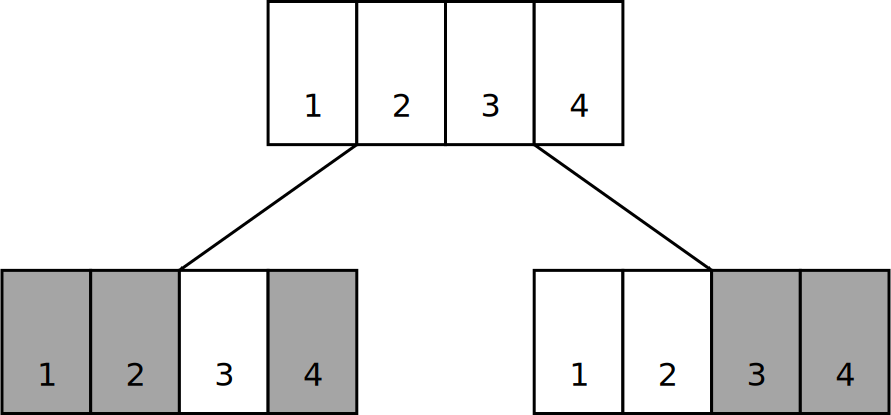
\includegraphics[width=0.5\linewidth]{images/cover_choice.pdf}
    \caption{When boards 1 to 4 are all uncovered, and a 7 is rolled, there are two possible valid coverings - covering boards 1, 2 and 4 (on the left), and covering boards 3 and 4 (on the right).}
    \label{cs1:cover_choice}
\end{figure}

Intuitively, this suggests that lower numbered boards are more valuable later in the game, since they increase the set of possible die rolls that a player can roll without ending the game. From this intuition, we develop two potential strategies for playing Shut the Box. The \emph{high-board strategy} is the strategy where the player always elects to cover the highest number board at each stage, while the \emph{low-board strategy} is the converse, where the player always elects to cover the lowest numbered boards at each stage.

When evaluating the effectiveness of these strategies, model checking is a suitable strategy. Since these strategies are deterministic, we may define DTMCs that model Shut the Box under these strategies, define the score of the game as a reward structure, and evaluate the expected score when the game terminates. However, we are also interested in the \emph{optimal} strategy - that is, the strategy which maximises the expected score of Shut the Box. Trying to enumerate and consider every possible strategy would be challenging, both conceptually and computationally. Instead, we consider the nondeterministic strategy, and derive an optimal strategy from here by choosing a series of actions in order to induce an optimal deterministic strategy. In order to achieve this, we consider a generalisation of a DTMC which supports nondeterminism.

\section{Background}
\label{cs1:stb_background}

We start by introducing Markov decision processes (MDPs) as described in \cite{forejt_automated_2011}, which are generalisations of DTMCs allowing for actions to be taken at each state, each leading to different probabilistic transitions between states. We then consider adversaries - resolutions of nondeterministic choice in MDPs - and briefly discuss how optimal adversaries are computed.

\subsection{Markov decision processes}
\label{cs1:mdps}
First, we define an MDP as a modification of a DTMC.

\begin{definition}
\label{cs1:def_mdps}

A Markov decision process (MDP) is a tuple $(S, \bar{s}, A, \delta, L)$, where $S$, $\bar{s}$ and $L$ have the same meanings as in Definition \ref{back:dtmc}. $A$ is the finite set of \emph{actions} on the MDP, while  $\mathbf{\delta} : S \times A \rightarrow Dist(S)$ is the new partial transition probability function, where pairs of states and actions are mapped to probability distributions denoting a transition to another state.

\end{definition}

For example, in a game of Shut the Box, $Act$ is the set of possible subsets of boards that the player can cover (such as the action of covering boards 3 and 5 simultaneously). Hence, $\mathbf{Steps}$ maps each state, including the current die value and the current set of uncovered boards, to the set of all possible covering arrangements along with the associated state transition.

Note here that, in general, a state may be associated to more than one action-distribution pair. Indeed, this is where nondeterminism is introduced into the MDP. In order to resolve this nondeterminism, we introduce the concept of adversaries.

\begin{definition}
\label{cs1:adversaries}

Given a \emph{finite} path $\omega = s_0 \rightarrow s_1 \rightarrow \dots \rightarrow s_n$, an adversary is a function $\sigma$ which maps each finite path to an action-distribution pair.

\end{definition}

A key remark on this definition is that adversaries make decisions depending on the entire execution history up to and including the state $s_n$, not just the state $s_n$ itself. However, we primarily consider \emph{memoryless adversaries}, where the adversary always picks the same choice in a given state. In particular, this adversary can be viewed as a map from states to actions. \gethin{with change in definition of Steps this is just a mapping to actions} Throughout the remainder of the dissertation, we only consider memoryless adversaries unless stated otherwise. We also remark that optimal adversaries for MDPs are non-randomised, so given a particular state the same action is always chosen. However this is no longer the case in concurrent models, which are discussed further in the third case study.

When an MDP is considered under an adversary, nondeterministic choice is resolved, and a DTMC is obtained. Hence, under a specific adversary, we can apply the model checking techniques introduced in Section \ref{back:prob_mod_check} to evaluate properties of an MDP.

Note that adversaries are often referred to using other names, depending on context, such as schedulers or policies. Throughout this dissertation, by convention we refer to adversaries when discussing the concept over general MDPs, and refer to strategies in the context of a particular game (analogous to a human developing a strategy while playing a game).

We defer discussion on how adversaries are generated until Section \ref{cs1:adversary_gen}. For now, we discuss how optimal values of probabilistic reachability properties are computed, then modify this process in order to provide an adversary which obtains this optimal value.

\subsection{Probabilistic reachability in MDPs}
\label{cs1:prob_reach_mdps}

In a similar manner to Section \ref{back:check-reach}, given an atomic proposition $a$, we define $T$ to be the set of states in some MDP $\mathcal{M}$ where $a$ holds.

Since MDPs allow for nondeterminism, we must consider a minimum and maximum probability of reaching $T$ from each state $s$ of the MDP, over all possible resolutions of nondeterminism. More precisely, for some atomic proposition $a$, and state $s$ (which may not necessarily be an initial state of the associated MDP) we denote these probabilities as $\mathbf{P}^{s}_{min=?} [\mathbf{F} \; a]$ and $\mathbf{P}^{s}_{max=?} [\mathbf{F} \; a]$ respectively. In order to calculate these probabilities, we introduce a method known as \emph{value iteration}, as described in [CITE VALUE ITERATION]. This method computes a sequence $(x^n_s)_{n \in \mathbb{N}}$, denoting the minimum or maximum probability of reaching $T$ from a given state $s$ within $n$ steps. This sequence then converges to an optimal value, yielding a reasonable approximation of the optimal value for large enough $n$.

First, we perform precomputation of several sets of states, very similarly to precomputation of $S^{yes}$ and $S^{no}$ in Definition \ref{back:S_yes}, where the minimum or maximum reachability probabilities are either 0 or 1. The details of these constructions are omitted and described further in Section 4.1 of \cite{forejt_automated_2011}. More formally, these precomputed sets are defined as follows.

\begin{definition}
\label{cs1:yes_no}

For a given MDP $\mathcal{M}$, with state space $S$ and atomic proposition $a$:

\begin{itemize}
    \item $S^{yes}_{min}$ is the set of states where $a$ eventually holds with probability 1, regardless of any nondeterministic choice.
    \item $S^{no}_{min}$ is the state of states where $a$ never holds in any subsequent reachable state, for some resolution of nondeterminism.
    \item $S^{yes}_{max}$ is the set of states where $a$ eventually holds with probability 1, for some resolution of nondeterminism.
    \item $S^{no}_{max}$ is the state of states where $a$ never holds in any subsequent reachable state, regardless of any nondeterministic choice.  
\end{itemize}
\end{definition}

We are now ready to define value iteration for calculating the minimum reachability probability for a set of target states $T$, via defining each element in the sequence $(x^n_s)_{n \in \mathbb{N}}$.

\begin{definition}
\label{cs1:value_iteration}

Given an MDP $\mathcal{M}$, with precomputed sets of states as described in Definition \ref{cs1:yes_no}, we have that:

\begin{equation*}
x^n_s = \begin{cases}
        1 & s \in S^{yes}_{min} \\
        0 & s \in S^{no}_{min} \\
        0 & s \notin (S^{yes}_{min} \cup S^{no}_{min}) \; \text{and} \; n=0 \\
        min_{A \in Act} \left( \sum_{s' \in S}\delta(s,A)(s') \cdot x^{n-1}_{s'} \right) & \text{otherwise} \\
    \end{cases}
\end{equation*}

\end{definition}

Using this method, optimal values can be obtained using an iterative process, and in particular the number of iterations required for a reasonable level of convergence can be determined during the algorithm's execution, such as terminating when the difference between two consecutive terms in the sequence is less than some pre-defined $\epsilon$. However, this specific approach is somewhat flawed, particularly when probabilities are initially small, or the sequence converges slowly. Several pieces of recent work have proposed alternative notions of convergence which address these issues, including the interval iteration algorithm described in \cite{haddad_interval_2018}, which considers upper and lower bounds on value iteration and proceeds until these bounds are sufficiently close together.

We now have a method of approximating $\mathbf{P}^{s}_{min =?} [\mathbf{F} \; a]$ and $\mathbf{P}^{s}_{max =?} [\mathbf{F} \; a]$, which we can then modify to produce not just the optimal values themselves, but a method for producing these optimal values, known as adversary generation.

\subsection{Adversary generation}
\label{cs1:adversary_gen}

In Definition \ref{cs1:value_iteration}, the inductive step is relatively simple: to find the maximum or minimum obtainable probability of reaching a state where $a$ holds within $n$ steps, we consider each possible action, consider each state it can transition to, then consider the probability of reaching a state where $a$ holds from each of these states, and finally choose the action where this value is minimised or maximised.

Hence, to compute the optimal adversary itself, we simply need to select the \emph{action} leading to the optimal value, rather than considering the value itself. Since our adversaries are memoryless, and hence defined as a mapping from states to actions, corresponding closely with value iteration. An example of this derivation is given below for calculating a minimum strategy.

\begin{definition}
\label{cs1:min_adv_generation}

Denote $Act(s)$ as the set of actions which are possible within a given state $s$. Then the strategy obtaining the minimum probability of reaching a state where some atomic proposition $a$ holds is given by

\begin{equation*}
    \sigma^{min}(s) = \text{arg min}_{A \in Act(s)} \left( \sum_{s' \in S} \delta(s, a)(s') \cdot \mathbf{P}^{s'}_{min =?} [\mathbf{F} \; a]\right)
\end{equation*}

\end{definition}

A slight modification of this technique is required for the maximum reachability case. To justify this, consider the following example:

\begin{example}
\label{cs1:bad_valit_example}

Consider the MDP presented in Figure \ref{cs1:bad_mdp_figure}. While in state $s_0$ or $s_1$, the $stay$ action will transition between $s_0$ and $s_1$, while the $exit$ action will transition to the goal state, $s_2$, and consider obtaining $\sigma^{max}(s_0)$ by replacing "min" with "max" in Definition \ref{cs1:min_adv_generation}. The $stay$ and $exit$ actions both have the same maximum value, so either may be selected, and similarly for $\sigma^{max}(s_1)$. But if $\sigma^{max}(s_0) = \sigma^{max}(s_1) = stay$, then the DTMC induced by $\sigma^{max}$ never reaches $s_2$, even though this occurs with probability 1 by selecting the $exit$ action.
\begin{figure*}

\centering
\begin{tikzpicture}[->,>=stealth',shorten >=1pt,auto,node distance=3.5cm,
    scale = 1,transform shape]

\node[state,initial] (s_0) {$s_0$};
\node[state] (s_1) [right of=s_0] {$s_1$};
\node[state,accepting] (s_2) [below of=s_1] {$s_2$};

\path (s_0) edge              node {$stay, 1$} (s_1)
    (s_1) edge              node {$stay, 1$} (s_0)
    (s_0) edge              node {$exit, 1$} (s_2)
    (s_1) edge              node {$exit, 1$} (s_2);

\end{tikzpicture}
\caption{An MDP where the naive approach to adversary generation does not succeed.}
\label{cs1:bad_mdp_figure}
\end{figure*}
\end{example}

We may still use a similar idea as for minimum adversary generation, but in order to avoid the issue presented in Example \ref{cs1:bad_valit_example}, a slight modification is required to prioritise actions which arrive at the set of target states.

Given a specific optimal adversary $\sigma$, computing the reachability probability of an MDP under the adversary is fairly simple, by considering the DTMC induced by $\sigma$ and using the techniques introduced in Section \ref{back:check-reach}. But the converse, that we have shown in this section, is potentially more surprising - given an optimal value for a reachability probability, an adversary can be constructed that obtains this optimal value, during the process of value iteration, with minimal additional computation.


\section{Analysis (3 pages)}

Collect some data, show the results.

\hrule

\Blindtext

\Blindtext

\Blindtext

\section{Evaluation(2 pages)}

The key section - use the results from model checking to answer questions about the game (for instance, to examine the difficulty and/or complexity of a game).

\hrule

\Blindtext

\Blindtext